\documentclass[article,9pt,twocolumn,twoside]{rilabRxiv}
% Use the documentclass option 'lineno' to view line numbers
\setlength{\marginparwidth}{2cm}
\usepackage[textsize=tiny,colorinlistoftodos]{todonotes} % comments in margins
\definecolor{cornflowerblue}{rgb}{0.39, 0.58, 0.93}
\usepackage{blindtext}

\usepackage{hyperref}
%interwordspace: \the\fontdimen2\font \\

%interwordstretch: \the\fontdimen3\font \\

%emergencystretch: \the\emergencystretch\par
%\blindtext

%%%%%%%Add comments in color
\newcommand{\ms}[1]{{\small \textcolor{green}{#1}}}
\newcommand{\jri}[1]{{\small \textcolor{red}{#1}}}
\newcommand{\citex}[1]{{\small \textcolor{red}{CITE(#1)}}}
\newcommand{\X}{{\textcolor{red}{X}}}

\newcolumntype{b}{X}
\newcolumntype{s}{>{\hsize=.5\hsize}X}

% Set supplement numbers to S and start counting newly
\newcommand{\beginsupplement}{%
        \setcounter{table}{0}
        \renewcommand{\thetable}{S\arabic{table}}%
        \setcounter{figure}{0}
        \renewcommand{\thefigure}{S\arabic{figure}}%
     }


\title{Method of Analysis of Multi-parent Mapping Populations Affects Detection of QTL}

\author[$\ast$,1,2]{Odell, S. G.}
\author[3]{Praud, S.}
\author[2,4,5]{Ross-Ibarra, J.}
\author[1]{Runcie, D.}


\affil[1]{Dept. of Plant Sciences, University of California, Davis, CA, USA}
\affil[2]{Dept. of Evolution and Ecology, University of California, Davis, CA, USA}
\affil[3]{Limagrain, Chappes, France}
\affil[4]{Center for Population Biology, University of California, Davis, CA, USA}
\affil[5]{Genome Center, University of California, Davis, CA, USA}


\keywords{QTL, MAGIC}

\runningtitle{Running title} % For use in the footer

%% For the footnote.
%% Give the last name of the first author if only one author;
% \runningauthor{Odell}
%% last names of both authors if there are two authors;
% \runningauthor{FirstAuthorLastname and SecondAuthorLastname}
%% last name of the first author followed by et al, if more than two authors.
\runningauthor{Odell \textit{et al.}}

%%% Abstract %%%%%%%%%%%%%%%%%%
\begin{abstract}
The search for quantitative trait loci (QTL) that explain complex traits such as yield and drought tolerance has been ongoing in all crops. Methods such as bi-parental QTL mapping and genome-wide association studies (GWAS) each have their own advantages and limitations. Multi-parent advanced generation inter-crossing (MAGIC) contain more recombination events and genetic diversity than bi-parental mapping populations and reduce the confounding effect of population structure that is an issue in association mapping populations. Here we discuss the results of using a MAGIC population of doubled haploid (DH) maize lines created from 16 diverse founders to perform QTL mapping, comparing QTL identified using a 600K SNP array to those found using founder probabilities and haplotype probabilities generated by determining the regions of the MAGIC DH lines that were derived from the 16 founders and by identifying regions of identity-by-descent (IBD) between the 16 founders, respectively. The three methods have differing power and resolution for detecting QTL for a variety of agronomic traits. This highlights the importance of considering different approaches to analyzing genotypic datasets, and shows the limitations of binary SNP data for identifying multi-allelic QTL. A closer look at a well-characterized flowering time QTL, qDTA8, which cotains \emph{vgt1} and \emph{vgt2} highlights the strengths and weaknesses of each method and suggests a potential epistatic interaction.

\end{abstract}
%%%%%%%%%%%%%%%%%%%%%%%%%%

\DeclareRobustCommand{\rchi}{{\mathpalette\irchi\relax}}
\newcommand{\irchi}[2]{\raisebox{\depth}{$#1\chi$}} % inner command, used by \rchi
\setboolean{displaycopyright}{true}

\begin{document}

\maketitle
\thispagestyle{firststyle}
%\firstpagefootnote
\correspondingauthoraffiliation{
Dept. of Plant Sciences and Dept. of Evolution and Ecology, University of California, Davis, CA, USA
E-mail: sgodell@ucdavis.edu}
\vspace{-11pt}%

\section{Introduction}
%\subsection{First part}
\lettrine[lines=2]{\color{color2}T}{}he study of evolutionary quantitative genetics requires the ability to link differences in phenotype to genotypic variation. Natural and artificial selection act on phenotypes, but only heritable phenotypic variation will result in changes in population means. Maize presents an excellent model organism to quantitative genetics due to the combination of extensive genetic and phenotypic resources, and the ability to create mapping populations. In addition, maize is one of the most widely produced crops in the world and is a major source of calories for millions of people. Decades of research into maize genetics have resulted in the identification of many quantitative trait loci (QTL) that explain variation in phenotypes such as yield, flowering time, and plant height (\citep{RN3};\citep{RN1};\citep{RN7}). Such traits are extremely agronomically important. They are also crucial plant phenotypes in terms of fitness and local adaptation.
Researchers have been able to discover large-effect QTL for a number of agronomic traits through the use of different types of mapping populations \citep{RN8}. The choice of any population comes with associated advantages and limitations. In particular, they tend to vary in two main characteristics: (1) their ability to capture genetic diversity and (2) their power to detect QTL of small effect. Multi-parent Advanced Generation Intercross (MAGIC) populations have been used in breeding to increase the genetic diversity and number of recombination events included in a mapping population compared to biparental populations \citep{RN5};\citep{RN5};\citep{RN31};\citep{RN4};\citep{RN24}. Compared to genome-wide association panels, MAGIC populations have more power to detect rare alleles (i.e. alleles that are only present in one of the parents) and can better estimate allelic effects because the crossing scheme increases the frequency of all parental alleles to be approximately equal. Simulations of an 8-parent MAGIC population showed that sample sizes of 300 could detect QTL accounting for 12\% of variance with a power of 82\% \citep{RN4}. Lastly, a MAGIC population avoids confounding due to population structure that is encountered with GWAS because the pedigree of the lines is known.
In this study, we utilized a MAGIC population of 325 doubled-haploid lines derived from 16 inbred maize parents developed by Limagrain to understand how methods of representing genotypic data can impact the identification of QTL. Extensive genetic resources already exist for maize, but do not possess the same diversity and statistical power as the Limagrain MAGIC population. A maize nested association mapping (NAM) population exists, consisting of RIL populations derived from 25 inbred parents crossed to B73 \citep{RN11}.  Only two inbred parents overlap between the NAM and Limagrain MAGIC populations (B73 and Oh43), and compared to the NAM, the MAGIC population can have similar power to the NAM using half the number of samples \citep{RN4}. Likewise, another maize MAGIC population has previously been created, which overlaps by three parents (A632, B73, and B96) \citep{RN4}. However, the previous MAGIC is derived from 8 inbred maize parents instead of 16, and consists of RILs, not doubled haploids, so some residual heterozygosity may exist.  For these reasons, the Limagrain MAGIC population has great potential to reveal new insights into the genetic control of quantitative traits in maize. It also serves a reliable standard for QTL mapping method comparision because DH lines were used and the crossing scheme ensured that there is a reasonably even distribution of the 16 founders within the population (supplemental figure?)

In addition to the choice of mapping population, the choice of how to represent genetic information through association and QTL mapping can impact the power of a study to detect and analyze QTL. The method of association mapping uses panels of many diverse lines and uses markers, usually SNPs, to tag regions that are in linkage disequilibrium. This method, hereafter referred to as $GWAS_{SNP}$ utilizes historical recombination that has occurred since the lines of the panel diverged from one another. Most often with this method the SNPs represent a small region of the chromosome that is in tight LD with that SNP, and each site is bi-allelic, with either a reference or alternate allele.
The method of QTL mapping using linkage blocks created from the recombination that occurred over the course of producing the mapping population. Markers are used to represent larger linked chromosome segments, and the amount of recombination and size of chromosome segement determines the resolution of any identified QTL. In these mapping populations, the markers used can be said to represent the founder identity of that region, or which parent of the population that segment of chromosome was derived from. We will refer to this method hereafter as $QTL_F$ As a result, each marker can be bi- or multi-allelic dependent on how many founders were used in the making of the population. If there are more than two founders, or if not all markers segregate between two founders, one must infer the founder identity recombination points of chromosome regions. This is often done using a Hidden Markov Model (HMM). HMMs calculate the probability of being in a particular "hidden" state (here the founder identity) given the observed state (here the genotyped SNP) []. This method can also take into account a decent amount uncertainty stemming from genotyping error and other sources. [Discuss previous papers and attempts to do this]

The two method of representing genotype data described above make the assumption that for each genotyped marker, there are either two distinct alleles in the population ($GWAS_{SNP}$) or as many alleles as there are founders $QTL_F$. The latter assumption, although very possible for biparental mapping populations, becomes increasingly unlikely as the number of founders increases. In the case of the Limagrain MAGIC population, it seems improbable that each marker possesses 16 distinct alleles. This is because the founders used in a population are related to one another with varying degrees of distance, and therefore most likely share regions that are in identity-by-descent (IBD). IBD regions are segments of the genome that are genetically similar between individuals as the result of the individuals inheriting the segment from a common ancestor []. [Maybe talk about methods of determining IBD regions?] Information on haplotypes shared between two or more founders can be encorporated into QTL mapping. This method, hereafter referred to as $QTL_H$, allows the number of alleles at each marker to vary anywhere from two to the total number of founders (here 16). This has the potential to increase statistical power by reducing the number of tests.

Many previous studies have use variations of these methods to identify QTL, and some have directly compared them... To our knowledge, our method of converting genotype data into haplotypes, $QTL_H$ has not been done previously.

\subsection{A case study of \emph{qDTA8}}
Flowering time is a highly important trait. In addition to being a crucial agronomic trait, it is a large part of local adaptation for annual plants such as maize, ensuring that individuals can reproduce within the growing season of their environments [cite?]. Flowering time in maize has been shown to be a highly polygenic trait [cite] controlled by many, mostly small-effect loci. The relatively large effect of \emph{vgt1} compared to most other identified maize flowering time QTL has made it a target of a great deal of study. As a naturally-occuring variant, the frequency of the early-flowering allele of \emph{vgt1} has been shown to closely follow a latitudinal gradient, suggesting that there has been selection on \emph{vgt1} that allowed maize to spread to higher latitudes [cite Navarro?].

The flowering time QTL, \emph{vgt1} has been identified in multiple populations [cite]. Previous research by [cite] has shown that variation in flowering time at this site is strongly correlated with a MITE insertion within a conserved non-coding sequence about 70 kb upstream of a major flowering time regulatory gene, \emph{ZmRAP2.7} [cite], with the presence of the MITE associated with an earlier flowering time. Within maize heterotic groups, Flint maize lines tend to possess the early-flowering allele of \emph{vgt1} (\emph{MITE+}), while dents (such as B73) tend to carry the late-flowering allele(\emph{MITE-}) [cite?]. It is hypothesized that the MITE represses expression of \emph{ZmRAP2.7}, possibly due to change in methylation around the insertion [cite]. It has been shown that there a differentially-methylated regions between B73, landrace maize, and teosinte [cite]. However, the MITE has not been experimentally shown to cause a decrease in \emph{ZmRap2.7} expression and results in earlier flowering. Further, there has been some evidence of epistatic interactions, potentially with another flowering time QTL, \emph{vgt3} which can impact the effect of the QTL (Alain Charcosset, personal communication). However, a recent study using multiple multi-parent populations suggested that variation in the effect of \emph{vgt1} in different genetic backgrounds was due to local genetic variation surrounding \emph{vgt1}, rather than epistasis with distant loci. This finding suggests two possibilities: either (1) that the causal variant underlying \emph{vgt1} is some as-yet unidentified variant that is in tight, but imperfect linkage disequilibrium with the MITE insertion, or (2) that the MITE insertion directly impact flowering time, and that another variant nearby has a modifiying effect on the MITE.

Using a well-characterized flowering time QTL with a strong candidate causal variant that is variable in the population, we demonstrate differences between the three methods and explore potential epistatic interactions between \emph{vgt1} and other genetic variation in the population.
%%This is how you can \citet{hufford2012comparative} in line or as reference in
% the end \citep{bourne2017ten}.
%\subsection{Second part}
%\blindtext
\section{Materials and Methods}
\label{sec:materials:methods}
\subsection{Genotype Data}
The MAGIC population was derived from 16 inbred maize parents representing the
 diversity of European flint and U.S. dent heterotic groups. The 16 founder lines were crossed in a funnel crossing scheme, and then the resulting synthetic population was intercrossed for 3 generations with around 2000 individuals per cycle (Figure \ref{fig:figure1}A). Finally, 800 lines were selected from the synthetic population to create doubled haploids (DH), resulting in 550 MAGIC DH lines at the end of the process. The 16 founder lines and the MAGIC DH lines were all genotyped with the Affymetrix 600K Axiom SNP array \citep{RN13}. %In
%       addition, the 16 founder lines were sequenced with Illumina short-read
%       sequencing to a depth of [?]x, resulting in 45.4 millions SNPs and
%       5.4 indels after filtering using GATK best practices.
Total of 503,892 SNPs from 600K after filtering out invariant sites.  and [num] sites with missing data...

\subsection{Phenotype Data}
The MAGIC DH lines were crossed to a tester MBS84 to produce 325 hybrids. Due to variation in flowering time, a subset of the lines could not be crossed to the tester. The hybrids were grown in five different field locations in four different years, resulting in six distinct environment-years. The environment-years included Blois, France in 2014 and 2017, Nerac, France in 2016, St. Paul, France in 2017, Szeged, Hungary in 2017, and Graneros, Chile in 2015. For each genotype, two blocks of around 80 plants were grown under well-watered conditions. Measured phenotypes included days to anthesis (DTA), days to silking (DTS), plant height, percent harvest grain moisture, grain yield, and thousand kernel weight (adjusted to 15\% humidity), where values were averaged over blocks. Both flowering time phenotypes were measured as the sum of degree days since sowing with a base temperature of 6$^{\circ}$C (48$^{\circ}$F). Days to anthesis was considered as the growing degree days until 50\% of plants in a block were flowering at 25\% of the central tassel spike.

\subsection{Calculation and Validation of Founder Probabilities}
The package R/qtl2 \citep{RN2} was used to determine founder probabilities of the DH lines using the 600K genotype data and the cross type ``riself16''. Due to the fact that the actual crossing scheme and the cross type input into R/qtl2 differed, we wanted to assess the accuracy of the founder probabilities. This was done by simulating lines using the actual crossing scheme and assessing the performance of the calc\_genoprobs function of R/qtl2 in correctly identifying the founder genotype (Figure \ref{fig:figure1}). We developed an R package, magicsim (\url{https://github.com/sarahodell/magicsim}), to simulate the lines using the maize consensus genetic map from \citep{ogut2015joint} to generate approximate recombination rates across the chromosome. For 400 simulated lines, 99.6\% of SNPs were correctly assigned to the founder genotype. Sites were dropped for individual founders if the sum of probabilities for a particular founder across all MAGIC lines was less than 1 or if there where fewer than 5 MAGIC lines that had a probability greater than 0.8 for one of the founders. This was to ensure that effect sizes for individual founders could be effectively estimated. In addition, the founder probabilities were filtered for LD using an iterative approach where a SNP was dropped if the $R^2$ value of probabilities between it and the kept SNP was greater than 0.95. After filtering, a total of 4,578 sites were kept to represent segments of chromosomes with little recombination in the MAGIC DH lines.

\begin{figure*}[ht!]
\centering
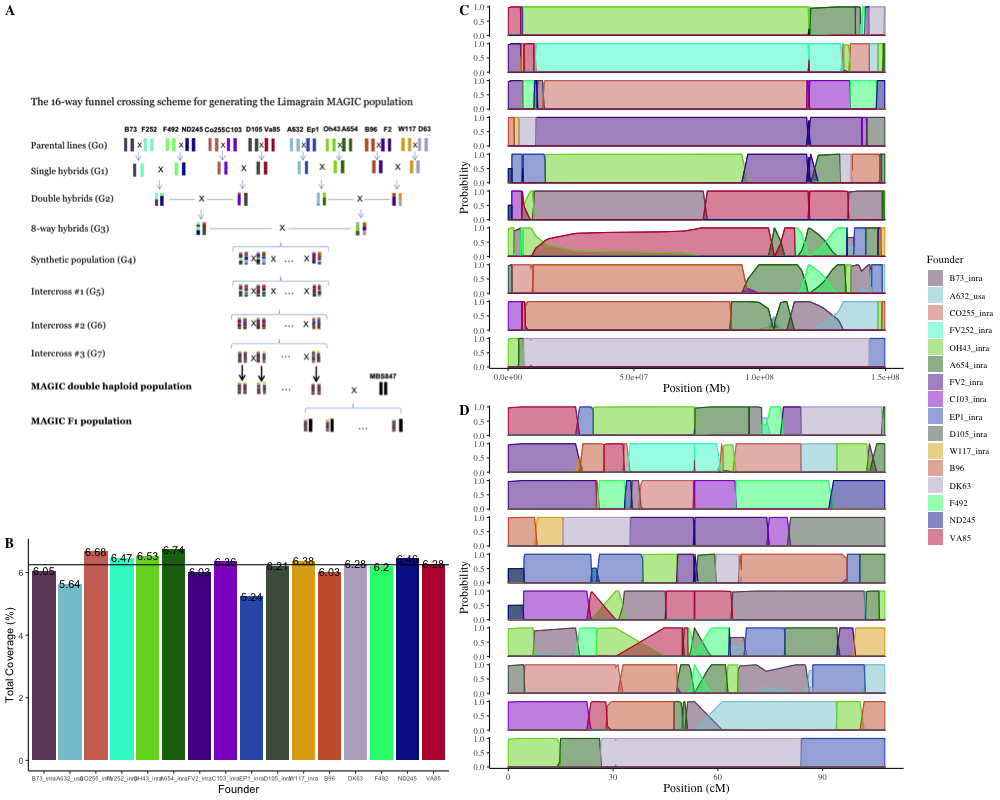
\includegraphics[width=\textwidth,height=14cm]{figures/Methods_Fig1.png}
\caption{\textbf{Structure, diversity, and founder representation of the MAGIC population}(\textbf{A}) The crossing scheme of the MAGIC population. (\textbf{B}) Founder probabilities for 10 MAGIC DH lines on chromosome 10 in physical distance. (\textbf{C}) The number of unique haplotype groups among the 16 founder lines across chromosome 10. (\textbf{D}) Founder probabilities for 10 MAGIC DH lines on chromosome 10 in genetic distance.}
\label{fig:figure1}
\end{figure*}

\subsection{Calculation of Identity-by-Descent and Haplotype Probabilities}
The use of founder probabilities makes the assumption that all 16 founders have distinct haplotypes. This assumption is not realistic, especially considering the known varying degrees of relatedness between the founders. The identification of regions of shared genetic sequence between founder pairs would allow for the collapsing of founder probabilities into haplotype probabilities. These haplotype probabilities have the potential to increase statistical power by reducing the number of tests performed in QTL mapping. Areas of uncertainty in founder probabilities of the DH lines were associated with regions of identity-by-descent (IBD) between two or more founder lines in that region of the chromosome. IBD was measured from the 600K SNP data of the founders using the software RefinedIBD \citep{Browning459}.
%RefinedIBD requires no missing data, so the software PLINK was used to impute
%missing data without a reference, which sets all missing sites to the allele
%frequency of the alterante allele within the samples. In addition, only
%bi-allelic sites were kept for the calculation of IBD, resulting in a total of
%16.9 million SNPs for comparison of sequence similarity.
The resulting segments of pairwise IBD between each of the 16 founders were used to identify distinct haplotype blocks [elaborate, supplemental figure?]. Within blocks, the founder probabilities for founders that were in  IBD were summed to obtain haplotype probabilities. This resulted in haplotype blocks with the number of unique haplotypes within blocks ranging from 6 at the lowest and 16 at the highest. Sites were dropped for individual haplotypes if the sum of probabilities for a particular haplotype across all MAGIC lines was less than 1 or if there where fewer than 5 MAGIC lines that had a probability greater than 0.8 for one of the haplotypes. This was to ensure that effect sizes for individual haplotypes could be effectively estimated. The haplotype probabilities were filtered for LD using an iterative approach where, for all haplotype blocks with the same number of distince haplotypes,a SNP was dropped if the correlation of probabilities between it and the kept SNP was greater than 0.95. After filtering, a total of 11,105 sites were kept to represent haplotype blocks in the MAGIC DH lines.

%\subsection{Imputation of WGS Data}
%The founder probabilities obtained from the 600K genotype data of the founders
%and the MAGIC DH lines was used to impute the WGS data from the founders onto the
%325 MAGIC lines. This was done using a custom script which calculated the
%probabilities of a MAGIC line having the alternate allele at each site in the
%WGS data based upon the founder probabilities of the line and the alleles of the
% 16 founders at that site. Only sites with less than 25\%(?) missing data were
% kept for imputation.

\subsection{Association and QTL Mapping}
The R package GridLMM was used to run association mapping using the three different methods of representing the genotype data \citep{RN14}. The function GridLMM\_ML was used with the "ML" option.  The following three models were approximated by fitting each locus independently. The three methods differed in the $X$ matrix used in the mixed linear model. The model that encorporated the raw 600K SNP genotype data (hereafter referred to as $GWAS_S$) was:
\begin{equation}
\label{eqn:gridlmm1}
 Y = X_S{\beta_S} + Zu + \epsilon
\end{equation}

where $Y$ is the response variable, $X_S$ is an $n$ x $p$ genotype matrix with reference and alternate alleles represented as 0 and 1, respectively, $\beta_S$, is the effect size of the alternate allele, $Z$ is the design matrix, $u$ is the random effects, and $\epsilon$ is the error.GridLMM fit an $n$ x 1 matrix for each site $p$.

The model that encorporated the founder probabilities (hereafter referred to as $GWAS_F$) was:
\begin{equation}
\label{eqn:gridlmm2}
 Y = X_F{\beta_F} + Zu + \epsilon
\end{equation}
where $Y$ is the response variable, $X_F$ is a ($n$ x $p$) x $f$ matrix and $x_{fnp}$ is the probability that at site $p$, individuals $n$ was derived from founder $f$, $\beta_F$, is the effect size of each founder allele, $Z$ is the design matrix, $u$ is the random effects, and $\epsilon$ is the error. GridLMM fit an $n$ x $f$ matrix for each site $p$.

The model that encorporated the haplotype probabiliteis (hereafter referred to as $GWAS_H$) was:
\begin{equation}
\label{eqn:gridlmm3}
 Y = X_H{\beta_H} + Zu + \epsilon
\end{equation}
where $Y$ is the response variable, $X_H$ is a ($n$ x $p$) x $h$ matrix and $x_{hnp}$ is the probability that at site $p$, individuals $n$ has haplotype $h$, $\beta_H$, is the effect size of each haplotype allele, $Z$ is the design matrix, $u$ is the random effects, and $\epsilon$ is the error. GridLMM fit an $n$ x $h$ matrix for each site $p$.

 Significance cutoffs for p-values were obtained using permutation testing, taking the 5\% cutoff from 1000 randomized permutations for each method. Code for the analyses can be found [github link].
%We used the software GEMMA [reference] to build a mixed linear model to identify
% QTL due the faster run time of this software with larger datasets.

\subsection{Method Comparison}
The results of the three methods of identifying QTL were compared using two main criteria: (i) presence or absence of identified QTL peaks and (ii) the resolution of those QTL peaks. %QTL bounds were determined using a Likelihood Ratio Test (LRT) comparing models with and without the most signifant marker of a QTL peak as a covariate [code link]. Using the the signifance threshold determined previously from 1000 random permuations from GWAS and QTL mapping, the QTL bounds were called as the first 10kb windows moving outward along the chromosome from the covariate marker that did not contain any markers with a higher LRT p-value than the threshold.%
QTL support intervals were determined by identifying the most significant SNP for a QTL peak and demarcating the left and right bounds of the QTL as the left-most and right-most SNPs within a 100Mb window centered on the highest SNP that have a log10 p-value that is 2 log10 p-values below that of the highest SNP.

The presence and absence of QTL was compared across the three methods for each phenotype. A QTL was said to be identified across methods if the QTL support interval for that QTL overlapped between the three methods.

The effect of the method used on the size of QTL support intervals was investigated using the QTL which were identified by all three methods (n=40). The model constructed was:

\begin{equation}
\label{eqn:bounds}
 Support Interval Size = Environment QTL + Method + \epsilon
\end{equation}

The support interval size response variable was represented both in terms of physical distance (Mb) and genetic distance (cM).

The comparison of effect sizes between methods was done using the effect sizes estimates of the most significant site within the QTL support interval. For methods that did not identify a QTL detected in other methods, comparison of effect sizes used the site with the highest log10 p-value that overlapped with the QTL support interval from the method that did detect the QTL.

%\textbf{General}
%\begin{table}[htbp]
%\centering
%\caption{\bf Parameters and variables}
%\begin{tableminipage}{0.5\textwidth}
%\begin{tabularx}{\textwidth}{sb}
%\hline
% Variable & Description \\
%\hline
%$N_{anc}$ & Population size at equilibrium \\
%$N_{final}$ & Population size after 0.1 * $N_{anc}$ generations \\
%$N_{bottlenck}$ & Population size during bottleneck \\
%$\psi$ & Genetic background proportion \\
%$\sigma_m$ & Standard deviation of effect sizes of new mutations \\
%$V_S$ & Strength of stabilizing selection \\
%$V_{G0}$ & Genetic variance at equilibrium\\
%\hline
%\end{tabularx}
%  \label{tab:shape-functions}
%\end{tableminipage}
%\end{table}

%\subsection{Experiment 1}
%\blindtext

%\subsubsection{Experiment 2}
%This is an example equation

%\begin{equation}
%\label{eqn:fitness}
%w =exp [-\frac{(z-z_{opt})^2}{2V_S}]
%\end{equation}

%\blindtext
%%%%%%%%%%%%%%%%%%%%%%%%%%%%%%%%%%%%%%%%%%%%%%%%%%%%%%
\section{Results}
%%%%%%%%%%%%%%%%%%%%%%%%%%%%%%%%%%%%%%%%%%%%%%%%%%%%%%

\subsection{MAGIC Population}
Analysis of the MAGIC population showed that the overall representation of the 16 founders in the MAGIC DH lines was relatively even, with the highest percentage founder, A654, representing 6.741\% and the lowest percentage founder, EP1, representing 5.237\% (Supplemental Figure). Across individual regions of each chromosomes, however, 33\% of founder probability sites significantly deviated from null ($\rchi^2$ test p-value < 6.82e-07 (15 df)) (Supplemental Figure).
This may be due to these founders being in close IBD with another founder, resulting in uncertainty in the founder probablities. Another possible explanation is that there was selection against these founders during the breeding process.

The avergae linkage disequilibrium R50 for the population was XX...
The MAGIC population also showed significant patterns of linkage disequilibrium between chromosomes. XX pairs of SNPs in the 600K genotype data that came from different chromosomes had $R^2$ values of greater than 0.7. The distribution of these regions of inter-chromosomal LD were ...

\subsection{Simulation and Validation of Founder Probabilities}
Using the package magicsim, we simulated chromosome 10 for 1000 MAGIC DH lines following the crossing scheme used for the actual population. We then ran R/qtl2 on these simulated lines to obtain founder probabilities and compared these probabilities to the known founder identities of the simulated lines. In total, for sites for which R/qtl2 was able to assign founder probabilities (X\% of sites), the maximum probability founder matched the actual founder for 99.8\% of sites. This reinforced our confidence in the founder probabilties obtained from the actual data.
The founder probabilities determined using R/qtl2 were able to assign founders to the actual MAGIC DH lines with high confidence (>0.90) for [percentage] of the 10 chromosomes of maize.

\subsection{Identity-By-Descent and MAGIC Haplotypes}
The results showed that a total of [bp][cM] of genome were in IBD between at
least two different founders. The average size of an IBD segment between two founders was 140kb (0.51 cM) with a median of 122kb (0.46). Pairwise IBD segments sizes ranged from 8 kb (0.3 cM) to  673 kb (1.61 cM). The total percentage of IBD between two founders ranged from 0.0018\% (F492 and VA85) to 4.3858\% (B73 and A632), with an average of 0.06130\%. There were no IBD segments found for 18 of 120 possible pairwise founder combinations.  [Distribution across chromosomes]

Amount of IBD between the founders and the tester, MBS847


\subsection{Phenotype Data}
The distribution of the six measured phenotypes were approximately normal (Figure \ref{fig:figure2}).

\begin{figure}[ht]
\centering
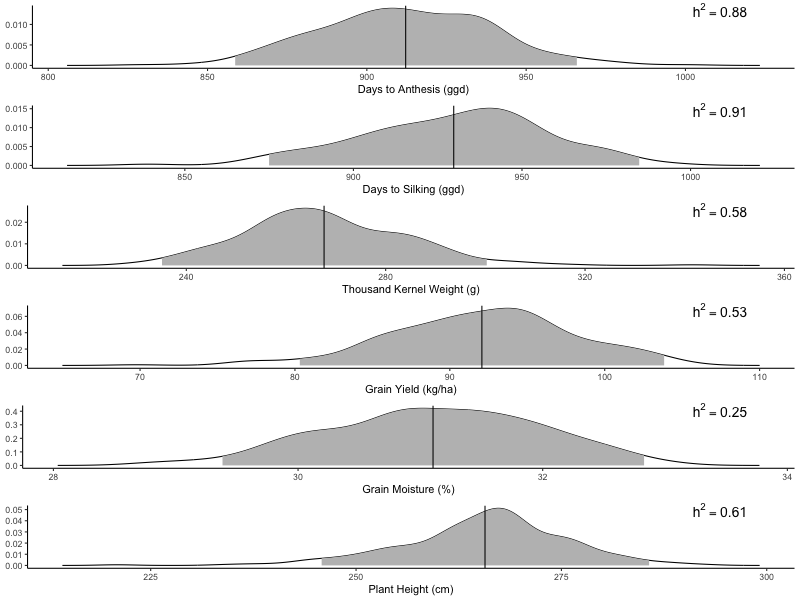
\includegraphics[width=\linewidth]{figures/Methods_Fig2.png}
\caption{\textbf{Distribution of phenotypes} The density plots of the six measured phenotypes. The vertical bar represents the mean, and the grey shading shows two standard deviations. The heritability of each trait is shown on the right.}
\label{fig:figure2}
\end{figure}

\subsection{QTL Mapping and Association Mapping}
The three methods varied in their ability to identify QTL.
Comparing methods within phenotype-environments, a total of 46 unique QTL were identified. 26 (57\%) of QTL were identified by all three methods. 6 QTL were found in both $GWAS_F$ and $GWAS_H$ and 1 QTL was found in both $GWAS_{SNP}$ and $GWAS_F$. 7, 3, and 3 QTL were found in only $GWAS_{SNP}$, only $GWAS_F$, and only $GWAS_H$, respectively (Supplemental Figure).

Comparing QTL across environments, there were 20 distinct QTL across all phenotypes, where QTL for a particular phenotype were considered shared across environments if their QTL bounds overlapped. 10 (50\%) of these across-environment QTL were found in more than one environment. 12 across-environment QTL were found using BLUPs and 2 of these QTL were not found in any individual environment. 6 (0 unique) QTL were found in Blois, 2014, 7 (1 unique) in Blois, 2017, 7 (3 unique) in Graneros, 2015, 5 (1 unique) in Nerac, 2016, 6 (3) in St.Paul, 2017, and 3 (0 unique) in Szeged, 2017. Only one QTL, qDTA8 (\emph{vgt1}) was found in all environments and the BLUPs.

Say something about the number of QTL found for different phenotype groups (i.e. FT, yield)?
%Do some count of QTL that are found with each method that don't have a peak in the other methods (qualitative for now)
In order to determine if comparison of methods was impacted by the semi-arbitrary choice of a 5\% significance threshold, we also used 1\% and 10\% permutation thresholds and checked if the number of QTL identified in each method changed dramatically by lowering or raising the significance threshold. $GWAS_F$ found the most QTL regardless of significance threshold, with $GWAS_H$ and $GWAS_{SNP}$ methods finding lower, but similar amounts of QTL. Individual QTL that were found in one method at the 5\% significance threshold usually became significant in other methods when at the 10\% threshold, indicating that the differences in the ability to detect these QTL between methods is mostly due to difference in power. There were, however, 10 QTL that appeared in one method and not in any others, mostly related to grain yield and thousand kernel weight traits. Whether these are due to false positives or true differences in the methods' abilities to identify QTL with different genetic architectures cannot be determined.

There was no significant difference in the resolution of those QTL between methods, both in physical (F-value = 0.5157, p-value = 0.5989) and genetic distance (F-value = 1.1658, p-value = 0.3165). Although on average, the physical and genetic size of $GWAS_{SNP}$ QTL bounds were larger than those of $GWAS_F$ and $GWAS_H$ QTL bounds, the difference was not significant and was most likely due to a few outliers. The average physical sizes of QTL bounds were 14.4 Mb (SE = 1.18 Mb) for $GWAS_{SNP}$, 12.8 Mb (SE = 1.07 Mb) for $GWAS_F$, and 13.4 Mb (SE = 1.09 Mb) for $GWAS_H$. The average genetic sizes of QTL bounds were 6.24 cM (SE = 0.353 cM) for $GWAS_{SNP}$, 5.85 cM (SE = 0.320 cM) for $GWAS_F$, and 5.51 cM (SE = 0.325 cM) for $GWAS_H$.

\subsection{Variation in Effect Sizes}
The effect sizes of QTL differed both across environments and between methods.

For QTL that were found with some methods and not others, we attempted to examine the effect sizes to see if they provided insight into the genetic architecture of the QTL. This might suggest some mechanism besides differences in statistical power that would explain the differences in QTL detection ability.

%SNP and founder
Looking at the effect sizes of most significant SNPs within QTL support intervals, the effect size of the founders with the alternate allele are different than the single effect size of the alternate SNP allele provided by $GWAS_{SNP}$. For QTL that were found with both $GWAS_{SNP}$ and $GWAS_F$, the effect sizes match up relatively better, but still show significant differences. These differences may be due to the fact that the most significant SNP in $GWAS_{SNP}$ and the most significant site in $GWAS_F$ may be different regions with slightly different LD structure.

QTL that were only found in the $GWAS_{SNP}$ method most likely have a bi-allelic causal variant. Looking at the founder effect sizes of the most significant site from the $GWAS_F$ within the $GWAS_{SNP}$ QTL support interval, the effect sizes have larger standard errors. This may be due to lower representation of some founders. It is also likely that the increased number of tests in the $GWAS_F$ method reduces statistical power when the true number of functional alleles is low.

%founder and haplotype
In most cases, the effect sizes of haplotypes average out the effect sizes of founders that are grouped together, weighted by the frequency of the founders in the MAGIC lines. For QTL that were identified in the $GWAS_H$ method and not the $GWAS_F$ method, the most likely reason for the difference is a failure of $GWAS_H$ to accurately represent the true haplotype structure of the QTL region. Generally, there were higher numbers unqiue of haplotypes in these cases, and the estimated effect sizes for haplotypes that grouped together more than one founder were quite different from the estimated effect sizes for those founders. Comparing effect sizes of QTL that were identified in $GWAS_H$ and not $GWAS_F$, there tended to be fewer unique haplotypes at these QTL regions and the effect sizes of haplotypes that grouped together more than one founder were similiar to the estimated effect sizes of those founders. This suggests that $GWAS_H$ was more successful in finding these QTL due to improved power when there were fewer functional alleles than founders.

On the whole, most QTL were found by all three methods, so there was limited abiity to draw reliable conclusions about underlying mechanisms that caused the methods to perform better or worse. Generally, the comparison of QTL detection and effect size estimates suggested that the methods failed and succeeded on a QTL-by-QTL basis. This is to be expected, as each QTL is the result of a distinct causal variant with a different number of alleles within the population.

\subsection{Variation around \emph{vgt1}}
One notable QTL that was identied by all three methods using BLUPs and nearly all individual environments was qDTA8, a large QTL on chromosome 8 that was strongly correlated with variation in days to anthesis, as well as days to silking. The support interval for this QTL overlapped with two previously characterized flowering time QTL, \emph{vgt1} and \emph{vgt2}. Research into these QTL has identified the underlying genes and several causal variants. For \emph{vgt1}, the earlier flowering phenotype is strongly correlated with a MITE insertion about 70kb upstream of the flowering time regulator, \emph{ZmRAP2.7}, an \emph{APETALA}-like transcription factor []. Evidence suggests that the presence of the MITE in a CNS upstream of \emph{ZmRAP2.7} results in changes in methylation, reducing the expression of \emph{ZmRAP2.7} []. As a negative regulator of flowering time, this reduced expression results in an earlier flowering phenotype []. The frequency of the MITE in maize populations follows a latitudinal gradient, suggesting that the early allele was selected for during the process of maize adaptation to temperate climates [].

The second QTL in this region, \emph{vgt2}, overlaps with the FT-ortholog \emph{ZCN8}, which has been shown to be the phloem-mobile flowering inducer, florigen. \emph{ZCN8} functions somewhere downstream of \emph{ZmRAP2.7}, and is negatively regulated by it. Variation in the promoter region of \emph{ZCN8} between temperate maize and teosinte suggests that earlier flowering alleles were under selection during the precess of maize domestication [].

The founders differ in the presence or absence of the MITE...

The effect sizes of vgt1 differ between founders and diverge from expectation (triple check that this is true)

The most significant SNP from $GWAS_SNP$ using BLUP scores for days to anthesis aligned strongly but imperfectly with the presence of the MITE. The correlation was still strong enough for the QTL to be significant. When looking at the founder effect sizes from $GWAS_F$, the estimates for founders are still quite different even if they share the MITE. This could be due to interaction with local genetic background or differences in estimation error due to lower representation of certain founders in the MAGIC lines at this region. Lastly, $GWAS_H$ groups founders together consistent with their allele at the MITE, but there are still far more than 2 distinct haplotypes (12?).



\begin{figure*}[hb!]
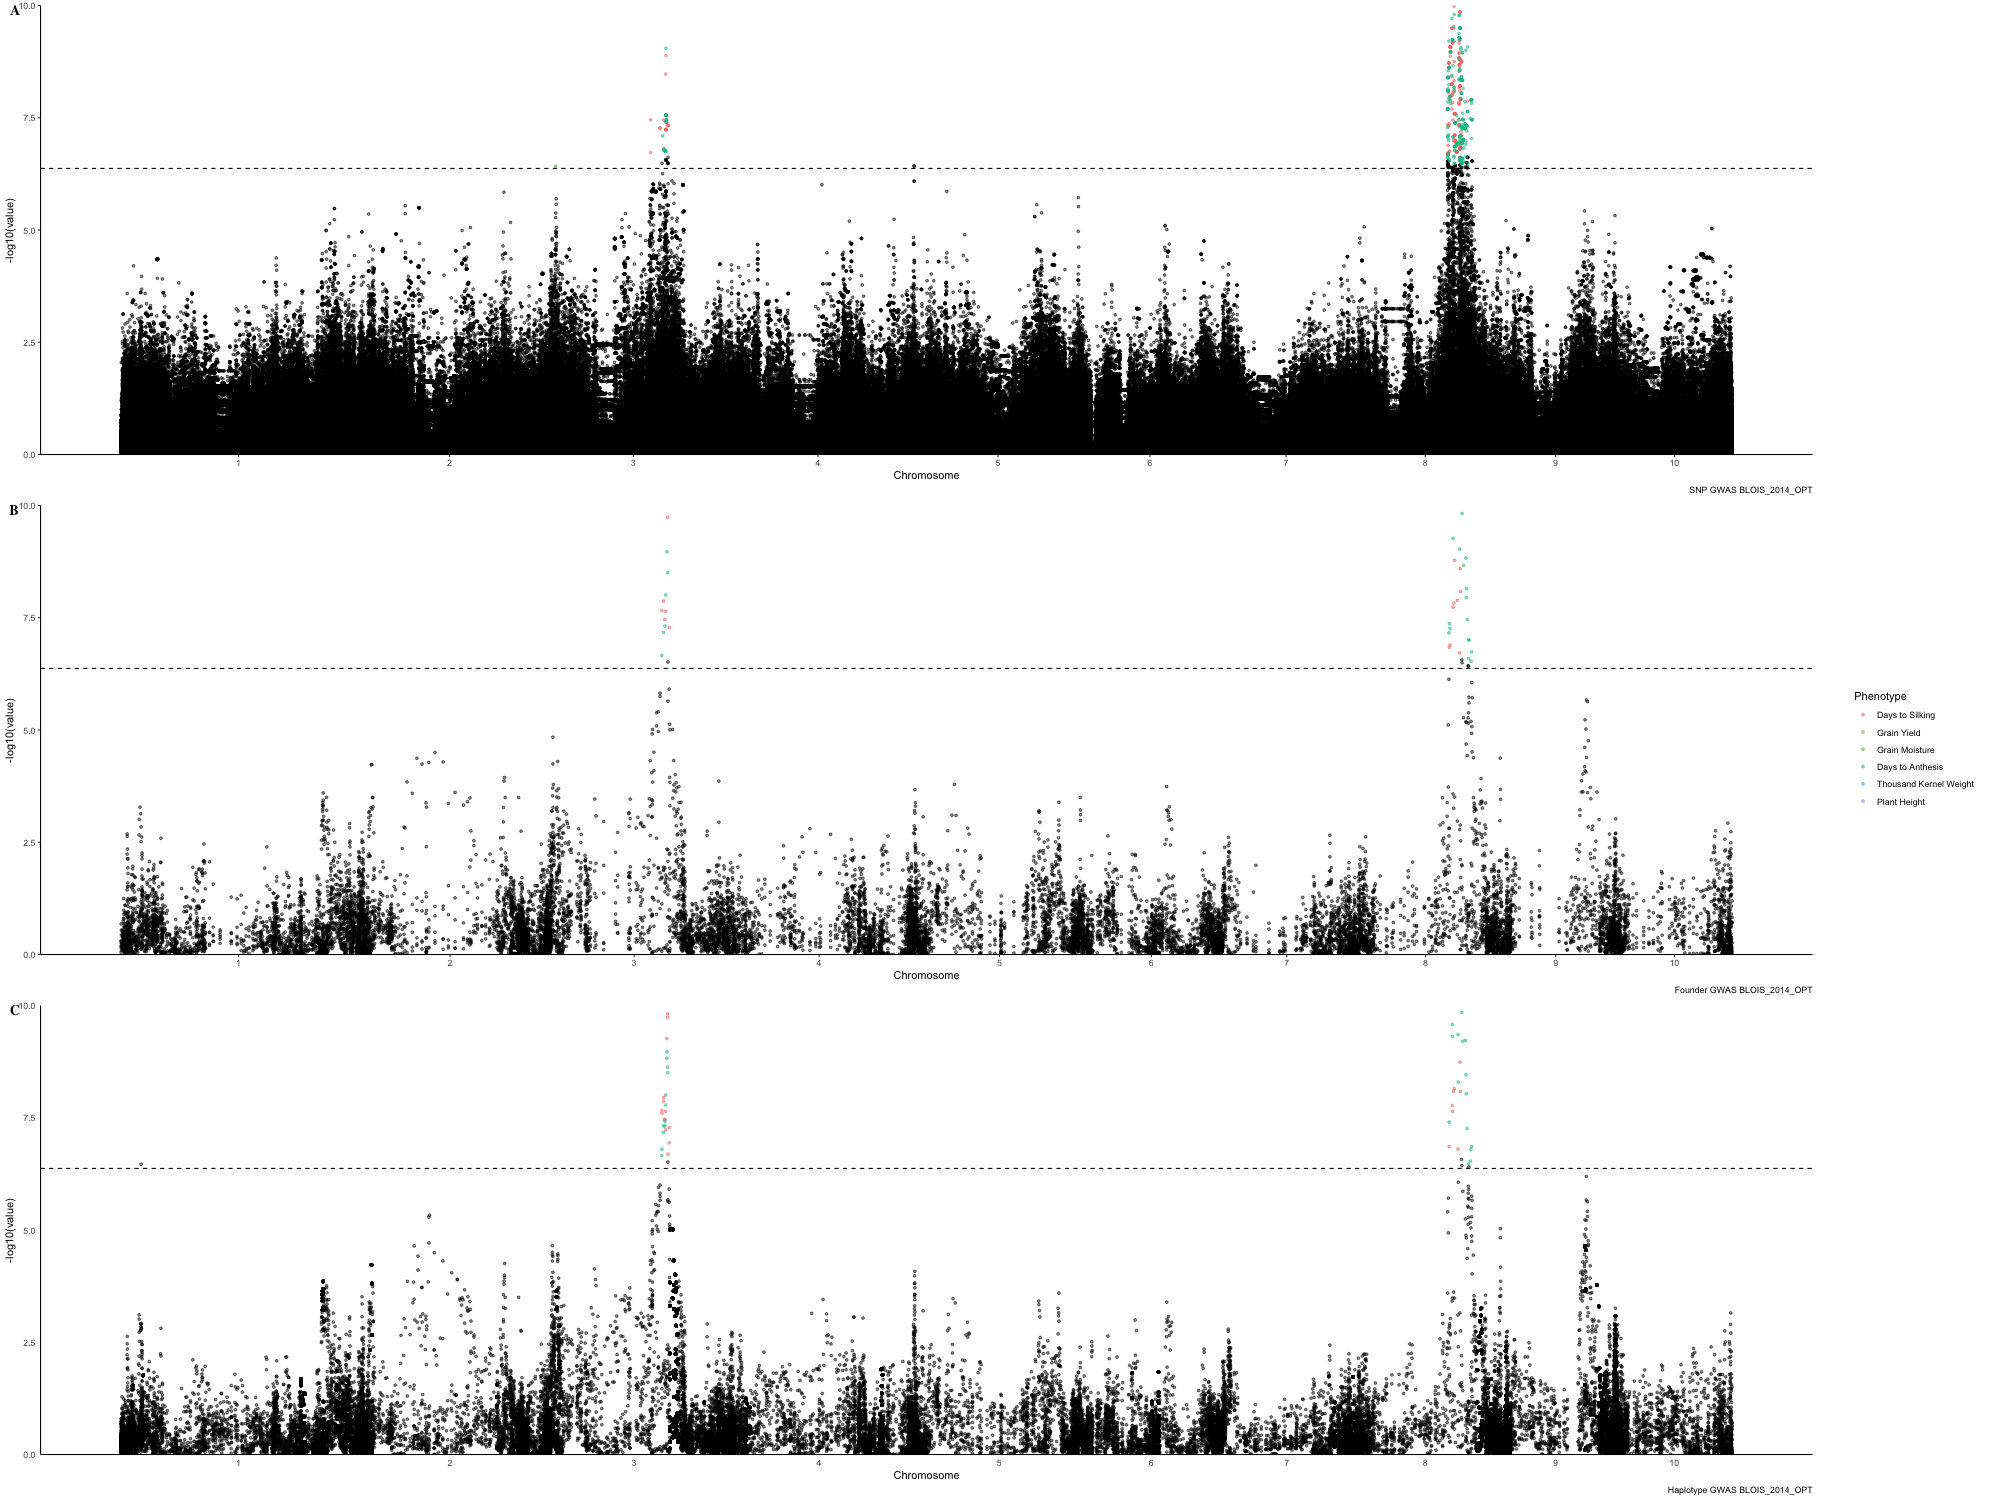
\includegraphics[width=\textwidth,height=14cm]{figures/Methods_Fig3.png}
\caption{\textbf{Results of three methods of QTL identification} Colored points represent signficant SNPs above the 5\% signficance threshold from 1000 random permutations \textbf{top} GWAS results using the 600K SNP array. \textbf{middle} Results from QTL mapping using founder probabilities \textbf{bottom} Results from QTL mapping using haplotype probabilities}
\label{fig:figure3}
\end{figure*}

Evidence of epistasis around \emph{vgt1}. Imperfect association between the presence of the MITE and the predicted effect size of the founder at vgt1 (Figure 4)



%\blindtext

%\blindtext
%\blindtext
%\blindtext
%\blindtext
%%%%%%%%%%%%%%%%%%%%%%%%%%%%%%%%%%%%%%%%%%%%%%%%%%%%%%
\section{Discussion}
%%%%%%%%%%%%%%%%%%%%%%%%%%%%%%%%%%%%%%%%%%%%%%%%%%%%%%
The results of using these three methods to identify QTL suggest that each has its own advantages and disadvantages in terms of how many and which QTL they can identify. If the goal of a study is to find as many QTL as possible, than it would be most useful to employ all three methods to maximize QTL identification.
The lack of significant difference in the genetic size of support intervals for the QTL found in the three methods suggests that the differences in QTL detection ability is more a result of differences in statistical power than a difference in ability to account for recombination events (?).


The GWAS methods should be most powerful at identifying QTL for which the causal variant is biallelic and the tagged SNP is in tight LD with the causal varaint. However, for multi-allelic QTL or QTL for which LD is low between tagged SNPs, this method begins to lose power. Founder probabilities increase the odds of detecting both QTL that are multi-allelic and QTL whose causal variant is not in tight LD with any one tagged SNP [Supplemental Figure?]. Lastly, haplotype probabilities potentially improve on the power of founder probabilities to detect QTL that meet the above criteria by reducing the number of test. However, haplotype probabilities also may obscure the signal of some QTL if founders are called as being in IBD with one another when they actually differ for the causal variant. Due to the fact that the founder and haplotype probabilities take into account recent recombination events, whereas the GWAS method only uses historical recombination, we predicted that founder and haplotype mapping would result in higher resolution around QTL peaks. Higher resolution QTL are ideal in that it makes it easier to narrow down candidate genes and potential causal variants when the significant window is smaller.

\subsection{IBD}
The lack of significant improvement of the $GWAS_H$ method relative to the others in some cases is most likely the result of the formation of haplotypes based off of sequence information that do not accurately reflect the functional haplotypes of the founder for particular phenotypes. Grouping of two or more founders into the same haplotype that do not share the same functional alleles underlying a QTL would result a decrease in the ability to accurately estimate haplotype effect sizes and a reduction in signal. It should also be noted that in the process of calculating pairwise IBD and assigning founders to haplotypes requires an inherently arbitrary significance threshold for calling founders as in IBD or not. In our case, this resulted in some incomplete haplotype graphs, meaning that in some cases, most, but not all founders grouped into the same haplotype were in pairwise IBD with the other founders in the haplotype.

\subsection{\emph{vgt1}}
One benefit of using founder and haplotype approaches lies in the potential to dissect the effects of individuals founders and/or haplotypes within QTL. This allowed us to look more closely at a well-characterized, large effect flowering time QTL, \emph{vgt1} and observe an interesting pattern of effect sizes that deviated from our expectations based on previous research. This opens up new areas of inquiry for future studies.


\subsection{another figure}
This is a full size figure (Figure \ref{fig:S1}) just add stars to the figure


\section{Acknowledgments}
We acknowledge the support of our coffee maker that made this work possible

\bibliography{magic_tex}

%\pagebreak
\onecolumn
\section*{Supplement}



\beginsupplement


\blindtext
\begin{figure*}[h!]
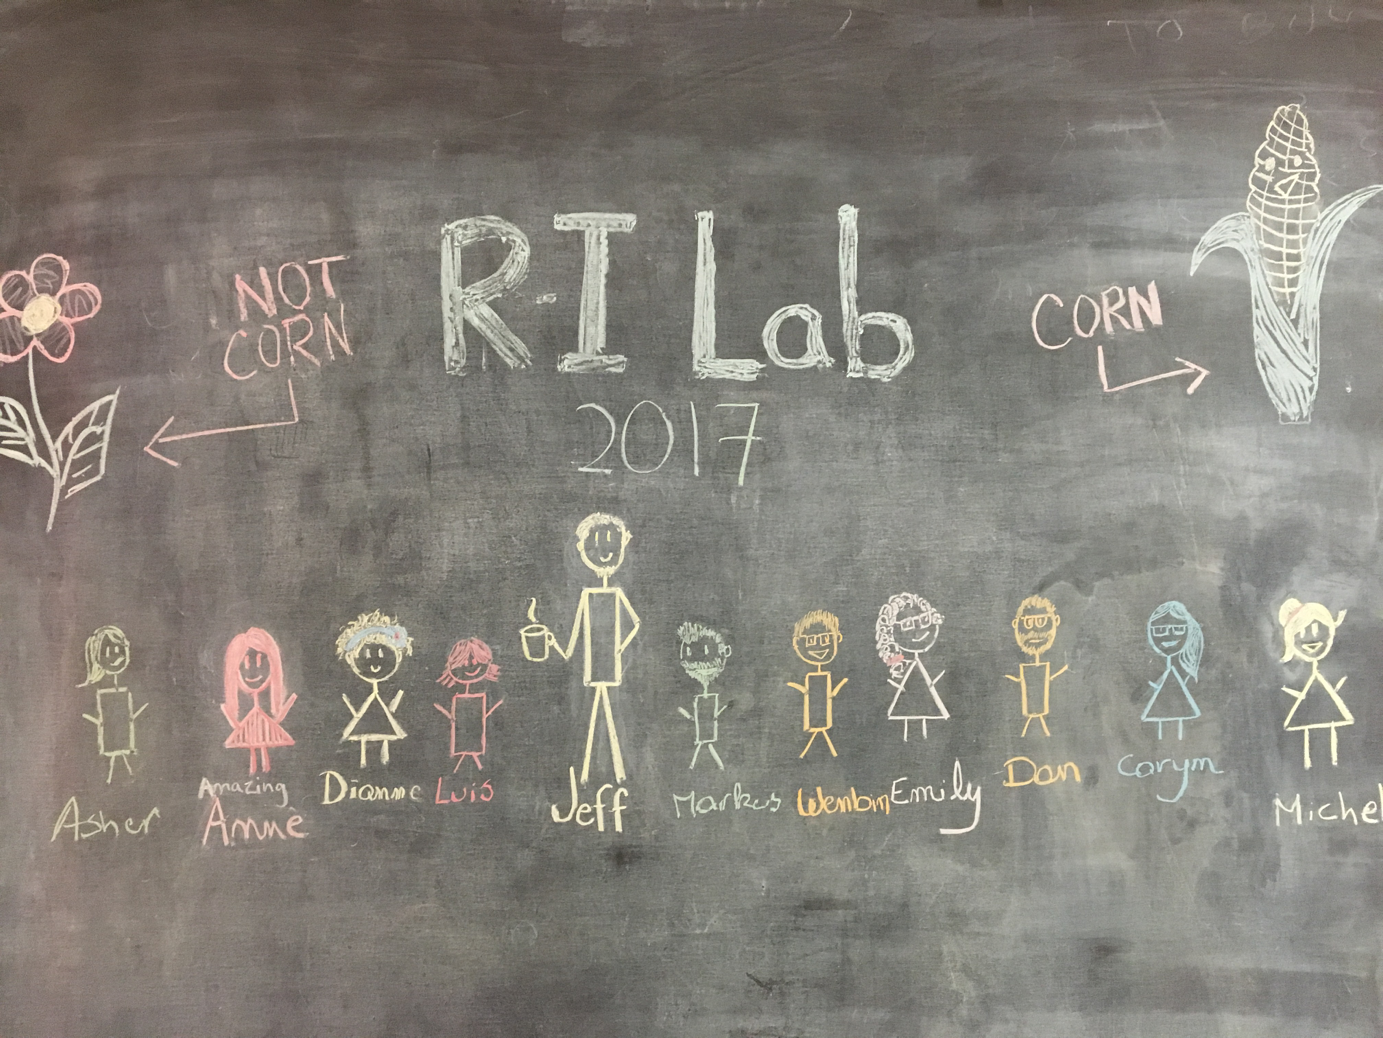
\includegraphics[width=.9\linewidth]{figures/lab_group.png}
\caption{\textbf{Supplemental figure} Test test test}
\label{fig:S1}
\end{figure*}
\pagebreak




\begin{table*}[htbp]
\centering

\caption{\bf Shrink a large table to fit the page}
%\begin{adjustbox}{totalheight=\textheight-2\baselineskip}
\begin{tableminipage}{\textwidth}
\begin{small}
\begin{tabularx}{\textwidth}{sb}
\hline
Parameter & Description \\
\hline
\textbf{Adaptation} & \textbf{Trait related parameters} \\
\hline
Time to optimum & Generations until new optimum is reached \\
Adaptation rate (haldane) & Adaptation rate until new optimum is reached. Calculated as $rate(h) = \frac{\frac{ln(x_2)}{sd_{x_{12}}}-\frac{ln(x_1)}{sd_{x_{12}}}}{t_2-t_1}$ \\
Final genetic variance & Genetic variance in the final generation \\
\textbf{Fixations} & \textbf{Mutations that fix after the optimum shift} \\
\hline
From new mutations (\#) & Sum of fixed mutations in the final population that were already segregating before  the optimum shift \\
From standing variation (\#) & Sum of fixed mutations in the final population that arose after the optimum shift \\
Max. effect size & Maximal effect size of all fixations \\
Mean effect size & Mean effect size of all fixations \\
Mean effect size of negative fixations & Mean effect size of negative mutations \\
Mean effect size of positive fixations & Mean effect size of positive mutations \\
Mean emergence time & Mean generation when a mutation arose that fixed in the last 0.1 N generations \\
Mean fixation time & Mean generation in which a mutation fixed \\
Min. effect size & Minimal effect size of all fixations \\
Negative (\#) & Sum of fixed mutations with negative effects in the final population \\
New/standing fixations & Ratio of mutations from new mutations vs. standing mutations  \\
Proportion negative & Proportion of negative fixations from all mutations \\
Positive (\#) & Sum of fixed mutations with positive effects in the final population \\
SD of effect sizes & Standard deviation of effect sizes of all fixations \\
SD of negative effect sizes & Standard deviation of effect sizes of negative fixations \\
SD of positive effect sizes & Standard deviation of effect sizes of positive fixations \\
Total (\#) & Sum of fixed mutations in the final population \\
\textbf{Sweeps} & \textbf{Mutations that fix faster than 99\% of neutral fixations} \\
\hline
Hard sweeps (\#) & Sum of selective sweeps from new mutations \\
Proportion of hard sweeps & Porportion of hard selective sweeps of all selective sweeps \\
Proportion of sweeps from standing & Proportion of selective sweeps from stainding variation of all selection sweeps \\
Sweeps (\#) & Sum of selective sweeps \\
Sweeps from standing variation (\#) & Sum of selective sweeps from mutations that were already segregating before  the optimum shift \\
Sweeps/fixations & Ratio of sweeps vs. fixations \\
\textbf{Segregating sites} & \textbf{Mutations that segregate in the final generation} \\
\hline
Max. effect size & Maximal effect size of segregating sites \\
Mean effect size & Mean effect size of segregating sites \\
Mean effect size of negative sites & Mean effect size of segregating sites with negative effects \\
Mean effect size of positive sites & Mean effect size of segregating sites with positive effects \\
Mean frequency of all sites & Mean allele frequency of segregating sites \\
Mean frequency of negative sites & Mean allele frequency of segregating sites with negative effects \\
Mean frequency of positive sites & Mean allele frequency of segregating sites with positive effects \\
Min. effect size & Minimal effect size of segregating sites \\
Negative (\#) & Sum of segregating sites with negative effect \\
Positive (\#) & Sum of segregating sites with positive effect \\
Proportion of negative sites & Proportion of segregating sites with negative effect of all segregating sites \\
Standard deviation of effect sizes & Standard deviation of effect sizes of all segregating sites \\
Total (\#) & Sum segregating sites in the final generation \\
\hline

\end{tabularx}
  \label{tab:parameter_list}
  \end{small}
\end{tableminipage}

%\end{adjustbox}
\end{table*}


\end{document}
